\chapter{Evaluation of Sequence-based Recommender Systems}
\graphicspath{{Chapter04/Figures/}}
\label{chap:sequeval}

From the outcome of our systematic literature review on multicriteria recommender systems discussed in Chapter~\ref{chap:multicriteria}, it emerged that traditional approaches usually guarantee interesting results in well-known domains, such as movie recommendation, but they are not capable of capturing the temporal evolution of users' preferences~\cite{Campos2013}. However, different authors~\cite{Ding2005,Rendle2010,He2017} argue that movies watched recently provide more useful information about a certain user than those she consumed in a distant past. It is, in fact, reasonable to assume that a recent item may have a high influence on the choice of the next one.

A recommender system that exploits sequential data for predicting the sole next item that will be consumed by a user can be defined as \emph{sequential recommender}~\cite{Wang2015}. Several works related to sequential recommenders are available in literature, as discussed in Section~\ref{soa:sec:sequential}. For example, Zhou et al.~\cite{Zhou2004} exploited a sequential pattern mining algorithm for recommending which page to visit next in a website, while Rendle et al.~\cite{Rendle2010} relied on Markov chains for suggesting products considering previous purchases. Recently, He et al.~\cite{He2017} designed a recommender system capable of modeling how users' interests evolve over time.

While all these methods usually consider user preferences observed during the training phase as sequences, no temporal ordering is available at recommendation time, as only one item, or a list of items ranked by relevance, is suggested to users. Because of the popularity of CF techniques, most of sequential recommenders are based on such approaches~\cite{Quadrana2018}, but in principle it is also possible to design systems capable of analyzing sequences according to content-based methods.

% Introduce the problem of sequence generation
In general, even if the problem of creating a sequence of words starting from an initial one is a well-known task inside the natural language processing community~\cite{Jurafsky2008}, the idea of creating personalized sequences of items is less widespread in the context of recommender systems~\cite{Herlocker2004}. For this reason, it would be interesting to be able to exploit the temporal ordering not only during the training phase but also for generating sequences of recommended items, such as in the task of language modeling. Some solutions to this problem have already been proposed in industry, and also few researchers have discussed how to automatically construct music playlists~\cite{Chen2012} or suggest sequences of points-of-interest to tourists~\cite{Feng2015} starting from seed items. However, early studies conducted in this field lack of a common definition of the problem that they are trying to address. For example, \emph{session-based} recommenders only consider the last session of the current user~\cite{Ludewig2018}, while \emph{sequence-aware} ones also exploit the history of past sessions~\cite{Quadrana2018} and they can be considered equivalent to sequential recommenders. Furthermore, it is not clear if item repetitions are allowed in the suggestions or not.

In this chapter, we argue that it is possible to consider recommender systems capable of creating personalized sequences of an arbitrary length as a generalization of a sequential recommender because the latter is only able of creating sequences of length \emph{one}. In contrast to traditional approaches that usually create lists of items ranked by relevance, in the following we will define a recommender that exploits a temporal dimension both in the training and in the generation phase as a \emph{sequence-based} recommender, as it observes and suggests sequences of items meant to be consumed in a particular order.

% Evaluation framework for sequence-based recommenders
As discussed in Section~\ref{soa:sec:evaluation}, several evaluation protocols and metrics for analyzing novel recommenders via offline experiments are available, to capture the different aspects of the recommendation algorithm~\cite{Gunawardana2015}. However, the lack of a standardized way of performing such \textit{in vitro} experiments leads to results that are often incomparable~\cite{Jannach2015}. To the best of our knowledge, no evaluation framework for sequence-based recommender systems has already been proposed. Our motivating hypothesis is that, in the context of sequence-based approaches, traditional evaluation metrics need to be computed at the level of sequences instead of the level of users. Therefore, we shift our focus from the multicriteria nature of the input ratings to multicriteria evaluation approaches, that rely on the set of metrics to perform an offline comparison among different recommendation methods.

% Research questions
In our view, an evaluation framework consists of a methodology for performing an experimental comparison, a set of metrics, and a software tool that implements them. The main aim of this chapter is to address the following research questions and to introduce an offline evaluation framework for sequence-based recommender systems that we called Sequeval.

\begin{description}
\item[RQ2.1\label{seq:itm:rq1}] What is the formal definition of a sequence-based recommender system?
\item[RQ2.2\label{seq:itm:rq2}] How already established metrics can be extended and adapted for evaluating a sequence-based recommender system?
\item[RQ2.3\label{seq:itm:rq3}] Against which baselines a sequence-based recommender system can be compared?
\end{description}

Because our evaluation approach is agnostic with respect to the implementation details of the algorithms under analysis, it can be successfully exploited to also assess the performance of systems based on alternative recommendation methods~\cite{Costa2011} or dealing with unconventional categories of items, for example 3D movies~\cite{Pouli2015} or cultural digital contents~\cite{Albanese2011}, especially if they are supposed to be consumed by users in a sequential order. Besides, by openly releasing a Python implementation of Sequeval, we aim to encourage the use of the proposed framework as an attempt to standardize the evaluation of sequence-based recommender systems, mitigating the comparability problem in recommendation research.

The remainder of this chapter is organized as follows: in Section~\ref{seq:sec:sequence-based} we present the mathematical definition of a sequence-based recommender system; in Section~\ref{seq:sec:sequeval} we introduce Sequeval by describing its evaluation protocol, metrics, and implementation details; in Section~\ref{seq:sec:analysis} we perform an empirical analysis of the framework with two datasets. Finally, in Section~\ref{seq:sec:conclusion}, we formulate our conclusions.

\section{Sequence-based Recommender Systems}
\label{seq:sec:sequence-based}

% Definition of rating
Before analyzing the evaluation framework, we introduce the problem of recommending sequences and we provide an answer to \ref{seq:itm:rq1}. In a traditional recommender system, users express positive or negative preferences about a certain item. An item may be, for example, a product, a song, or a place. In contrast, we assume that when a user consumes or interacts with an item, she expresses an implicit rating about it. This assumption in the literature goes under the name of \emph{implicit feedback}~\cite{Herlocker2004}. Because we are also considering the temporal dimension to build the sequences, each rating is associated with a timestamp that represents the point in time when it was recorded.

\begin{definition}
Given the space of items $\mathcal{I}$, the space of users $\mathcal{U}$, the space of timestamps $\mathcal{T}$, a rating $\mathbf{r} \in \mathcal{R}$ is a tuple $\mathbf{r} = (\iota, \upsilon, \tau)$, where $\iota \in \mathcal{I}$ is the item for which the user $\upsilon \in \mathcal{U}$ expressed a positive preference at the timestamp $\tau \in \mathcal{T}$.
\end{definition}

% Definition of sequence
By relying on the set of ratings $\mathcal{R}$ available in the system, it is possible to construct the sequences that will be used to train and to evaluate the recommender. Each sequence only includes the ratings expressed by a single user. On the other hand, each user may produce several sequences.

The concept of \emph{sequence} is similar to the concept of \emph{session} in a traditional web interaction: if two ratings are distant in time more than an interval $\delta \tau$, then they belong to different sequences. Some ratings may be isolated and, for this reason, not part of any sequence. The most appropriate value for $\delta \tau$ depends on the domain: for example, in the POI recommendation scenario, it could be considered of a few hours as reported in \cite{Feng2015}.

\begin{definition}
A sequence $\mathbf{s} \in \mathcal{S}$ is a temporally ordered list of ratings $\langle \mathbf{r}_1,\allowbreak \mathbf{r}_2,\allowbreak \dotsc,\allowbreak \mathbf{r}_n \rangle$ created by a particular user $\upsilon \in \mathcal{U}$, i.e., for each $i$, $\mathbf{r}_i = (\iota_i, \upsilon, \tau_i)$ and $\tau_i < \tau_{i + 1}$.
\end{definition}

In Algorithm~\ref{seq:alg:generate}, we list the procedure for creating the set $\mathcal{S}$, given the set of users $\mathcal{U}$, the set of ratings $\mathcal{R}$, and a time interval $\delta \tau$. Please note that we do not allow the creation of sequences of length \emph{one} because they do not encode a meaningful temporal order.

\begin{algorithm}
\caption{Generation of the set $\mathcal{S}$, given $\mathcal{U}$, $\mathcal{R}$, and $\delta \tau$.}
\label{seq:alg:generate}
\begin{algorithmic}[1]
\REQUIRE $\mathcal{U} \neq \{\emptyset\} \land \mathcal{R} \neq \{\emptyset\} \land \delta \tau \doteq \tau_i - \tau_j$
\STATE $\mathcal{S} \gets \{\emptyset\}$
\FORALL{$\upsilon \in \mathcal{U}$}
\STATE $\mathbf s \gets \varnothing$
\FORALL{$\mathbf r_i \in \mathcal{R}_{\upsilon} : \tau_{i - 1} < \tau_i \land i > 1$}
\IF{$\tau_i < \tau_{i - 1} + \delta \tau$}
\IF{$\mathbf s$ is $\varnothing$}
\STATE $\mathbf{s} \gets \langle \mathbf r_{i - 1} \rangle$
\ENDIF
\STATE $\mathbf{s} \gets \mathbf{s} + \langle \mathbf r_i \rangle$
\ELSE
\IF{$|\mathcal{R}_{\mathbf{s}}| > 1$}
\STATE $\mathcal{S} \gets \mathcal{S} \cup \{\mathbf s\}$
\STATE $\mathbf{s} \gets \varnothing$
\ENDIF
\ENDIF
\ENDFOR
\ENDFOR
\RETURN $\mathcal{S}$
\end{algorithmic}
\end{algorithm}

% Definition of sequence-based recommender
A sequence-based recommender is a recommender system capable of suggesting a personalized sequence that is built starting from a seed rating $\mathbf{r}_0$, considering the example sequences already available in the system and the specific behavior of a certain user. The seed rating is characterized by a seed item $\iota_0$, a target user $\upsilon$, and an initial timestamp $\tau_0$. The seed item can be represented by any item that belongs to the catalog, but, more in general, it is a point in the space of items $\mathcal{I}$. For example, in the music domain, it~could identify not only a particular song, but also an artist, a genre, or a mood. The target user is the user to whom the sequence is recommended, while the initial timestamp represents the point in time in which the recommendation is created. The generated sequence is of a fixed length and it contains exactly $k$ ratings. Please note that if $k = 1$, we are dealing with a sequential recommender as defined in~\cite{Wang2015}.

\begin{definition}
Given a seed rating $\mathbf{r}_0 \in \mathcal{R} : \mathbf{r}_0 = (\iota_0, \upsilon, \tau_0)$, and a length $k \in \mathbb{N}$, a sequence-based recommender is the function $\mathrm{sequence} : \mathcal{R} \times \mathbb{N} \to \mathcal{S}$, i.e., $\mathrm{sequence}(\mathbf{r}_0, k) = \langle \mathbf{r}_1, \mathbf{r}_2, \dotsc, \mathbf{r}_k \rangle : \mathbf{r}_i = (\iota_i, \upsilon, \tau_i)$.
\end{definition}

Most sequence-based recommenders are based on probability models, and therefore they can be interpreted as a sampling function $\sigma$ applied to the conditional probability $P(\langle \mathbf{r}_1, \mathbf{r}_2, \dotsc, \mathbf{r}_k \rangle | \mathbf{r}_0)$:

\begin{equation}
\mathrm{sequence}(\mathbf{r}_0, k) = \sigma (P(\langle \mathbf{r}_1, \mathbf{r}_2, \dotsc, \mathbf{r}_k \rangle | \mathbf{r}_0))
\end{equation}

Using the chain rule, the sequence probability $P(\langle \mathbf{r}_1, \mathbf{r}_2, \dotsc, \mathbf{r}_k \rangle | \mathbf{r}_0)$ can be written as:

\begin{equation}
\label{seq:eq:chainrule}
\begin{split}
P(\langle \mathbf{r}_1, \mathbf{r}_2, \dotsc, \mathbf{r}_k \rangle | \mathbf{r}_0) = & P(\mathbf{r}_k | \langle \mathbf{r}_0, \dotsc, \mathbf{r}_{k - 1} \rangle) \cdot \\ & P(\mathbf{r}_{k - 1} | \langle \mathbf{r}_0, \dotsc, \mathbf{r}_{k - 2} \rangle) \dotsm P(\mathbf{r}_1 | \langle \mathbf{r}_0 \rangle)
\end{split}
\end{equation}

For example, in the case of a Markov chain, each rating depends on the previous one, i.e., $P(\mathbf{r}_k | \langle \mathbf{r}_0, \dotsc, \mathbf{r}_{k - 1} \rangle) =\allowbreak P(\mathbf{r}_k | \mathbf{r}_{k - 1})$:

\begin{equation}
P(\langle \mathbf{r}_1, \mathbf{r}_2, \dotsc, \mathbf{r}_{k} \rangle | \mathbf{r}_0) = P(\mathbf{r}_k | \mathbf{r}_{k - 1}) P(\mathbf{r}_{k - 1} | \mathbf{r}_{k - 2}) \dotsm P(\mathbf{r}_1 | \mathbf{r}_0)
\end{equation}

Thus, a sequence-based recommender system typically works by learning from a set of sequences $\mathcal{S}_{training}$ the conditional probability of the next rating $\mathbf{r}_{k}$ to the sequence of previous ones $\langle \mathbf{r}_0, \mathbf{r}_1 , \dotsc, \mathbf{r}_{k - 1} \rangle$, i.e., the factors of the right-hand side of Equation~\ref{seq:eq:chainrule}.
Sampling sequences directly from Equation~\ref{seq:eq:chainrule} would require computing the probabilities of all the $|I|^k$ possible sequences, where $|I|$ is the size of the vocabulary of items and $k$ is the length of the sequences. Since this becomes easily computationally unfeasible, we opt for a greedy approach, in which at each step we sample the next most likely item. 
A sampling function $\rho$ is defined to select a particular next rating from the previous ones at each step:

\begin{equation}
\mathbf{\hat{r}}_{k} = \rho(P(\mathbf{r}_{k} | \langle \mathbf{r}_0, \mathbf{r}_1, \dotsc, \mathbf{r}_{k - 1} \rangle))
\end{equation}

A trivial example of $\rho$ is the $argmax$ function, which simply selects the most probable next rating. In the following, we will assume that $\rho$ is implemented by a weighted random sampling function.

Algorithm~\ref{seq:alg:recommend} formalizes the procedure for generating a personalized sequence, given a seed rating $\mathbf{r}_0$, and a length $k$, i.e., it describes the sampling function $\sigma$. For $k$ times, the next rating of the recommended sequence is generated using the function $predict$. The function $predict : \mathcal{S} \to \mathcal{R}$ implements the sampling function $\rho$ and it returns the most probable next rating for the current input sequence. In practice, the sequence-based recommender system can estimate the probability that the next rating of the current sequence will include a particular item at a certain timestamp.

Please note that the greedy procedure described in Algorithm~\ref{seq:alg:recommend} is not the only way to create samples of sequences, and thus, the user of the evaluation framework or the designer of the recommendation method are free to define other ways and strategies for that end. 

\begin{algorithm}
\caption{Recommendation of a sequence of length $k$.}
\label{seq:alg:recommend}
\begin{algorithmic}[1]
\REQUIRE $\mathbf{r}_0 \in \mathcal{R} \land k > 0$
\STATE $\mathbf{s} \gets \langle \mathbf{r}_0 \rangle$
\FOR{$i = 1$ \TO $k$}
\STATE $\mathbf{r}_i \gets \mathrm{predict}(\mathbf{s})$
\STATE $\mathbf{s} \gets \mathbf{s} + \langle \mathbf{r}_i \rangle$
\ENDFOR
\RETURN $\mathbf{s} - \langle \mathbf{r}_0 \rangle$
\end{algorithmic}
\end{algorithm}

% Number of items and ratings
To compute some metrics that are part of the evaluation framework, it is necessary to know the number of items that are associated with a certain sequence. For this reason, we define the set $\mathcal{I}_{\mathbf{s}}$ as the set of items that are part of the sequence $\mathbf{s}$, and the set $\mathcal{R}_{\mathbf{s}}$ as the set of ratings that are part of the sequence $\mathbf{s}$. Therefore, $|\mathcal{I}_{\mathbf{s}}|$ is the number of distinct items available in $\mathbf{s}$, while $|\mathcal{R}_{\mathbf{s}}|$ represents the length of $\mathbf{s}$, i.e., the number of ratings available in $\mathbf{s}$.

% Example
For instance, we can suppose that the set of ratings $\mathcal{R}$ is equal to $\{(\iota_1, \upsilon_1, \tau_1),\allowbreak (\iota_2, \upsilon_1, \tau_2),\allowbreak (\iota_3, \upsilon_2, \tau_3),\allowbreak (\iota_1, \upsilon_1, \tau_4),\allowbreak (\iota_2, \upsilon_2, \tau_5),\allowbreak (\iota_3, \upsilon_1, \tau_6)\}$. Then, if we assume that the only pair of timestamps that violates the $\delta \tau$ constraint is $(\tau_4, \tau_6)$, we can create two sequences: $\mathbf{s}_1 = \langle (\iota_1, \upsilon_1, \tau_1),\allowbreak (\iota_2, \upsilon_1, \tau_2),\allowbreak (\iota_1, \upsilon_1, \tau_4) \rangle$, and $\mathbf{s}_2 = \langle (\iota_3, \upsilon_2, \tau_3),\allowbreak (\iota_2, \upsilon_2, \tau_5) \rangle$. The rating $(\iota_3, \upsilon_1, \tau_6)$ is not part of any sequence because it was created at some point in time later than $\tau_4 + \delta \tau$ and we do not have any subsequent rating expressed by $\upsilon_1$. We also observe that $|\mathcal{I}_{\mathbf{s}_1}| = 2$ and $|\mathcal{R}_{\mathbf{s}_1}| = 3$. We would like to recommend a sequence $\mathbf{s}$ of length \emph{two} to user $\upsilon_1$ starting from item $\iota_3$ at timestamp $\tau_{\mathbf{s}, 0}$. In fact, it is not required that the item $\iota_3$ already appeared in the sequences related to user $\upsilon_1$. A possible solution to this problem is to define $\mathbf{r}_{\mathbf{s}, 0} = (\iota_3, \upsilon_1, \tau_{\mathbf{s}, 0})$ and then to recommend $\mathbf{s} = \mathrm{sequence}(\mathbf{r}_{\mathbf{s}, 0}, 2) = \langle (\iota_2, \upsilon_1, \tau_{\mathbf{s}, 1}),\allowbreak (\iota_1, \upsilon_1, \tau_{\mathbf{s}, 2}) \rangle$, where $\tau_{\mathbf{s}, 1}$ and $\tau_{\mathbf{s}, 2}$ may be used to suggest when consuming the items.

\section{Sequeval Evaluation Framework}
\label{seq:sec:sequeval}

Comparing the performance of several recommenders with an experiment that involves a live system is not always feasible or appropriate. For this reason, it is necessary to first perform a preliminary evaluation in an offline scenario~\cite{Gunawardana2015}. In such a setting, we can assess the performance of the algorithms by comparing with baselines, understanding the strengths and weaknesses of those, and thus avoiding affecting real users negatively in their experience with the system. The results of an offline experiment will be less trustworthy than the ones obtained from an online study because there was no real interaction with the system~\cite{Turpin2001}, but they are usually exploited as the first stage in the preparation of the in~vivo experimentation.

Even if an offline study is only the first step in the process of evaluating a recommender, it is necessary to rely on a solid evaluation protocol and a set of well-defined metrics that are able to capture all the characteristics of the analyzed algorithm~\cite{Ge2010}. In the following, we will introduce an offline evaluation framework for sequence-based recommender systems that we called Sequeval.

Our framework is based on the concept of sequence as formalized in Section~\ref{seq:sec:sequence-based}. First, an initial dataset is transformed into a set of sequences following Algorithm~\ref{seq:alg:generate}. Then, the sequences are split between training and test sets. At this point, one or more external recommenders are plugged into the framework: they are exposed to the training sequences and they are asked to create suggested sequences starting from the same seeds of the test ones. A possible strategy for suggesting additional sequences is described in Algorithm~\ref{seq:alg:recommend}, but the user can define other approaches. Finally, considering the recommendations available, the framework can compute different evaluation metrics.

In details, Sequeval is made of an evaluation protocol, presented in Section~\ref{seq:sec:protocol}, a set of evaluation metrics, described in Section~\ref{seq:sec:metrics}, and a software implementation that is introduced in Section~\ref{seq:sec:implementation}.

\subsection{Evaluation Protocol}
\label{seq:sec:protocol}

% Splitting protocol
One of the first problems that an evaluation framework should consider is how to split the dataset between the training set and the test set. This task is not trivial, as it will deeply influence the outcome of the experimentation~\cite{Said2014}. Since we are dealing with sequences, we need to split the set of sequences $\mathcal{S}$ in a training and test set such that $\mathcal{S} = \mathcal{S}_{training} \cup \mathcal{S}_{test}$.

Several solutions to this problem are possible: a simple but effective one is to perform the splitting by randomly assigning sequences to these sets according to a certain ratio, typically the $80\%$ for training and the $20\%$ for testing. If the number of sequences available is limited, it is necessary to perform a cross-validation. Another possibility is to identify an appropriate point in time and to consider all the sequences created before it as part of the training set, and after it as part of the test set. This protocol simulates the behavior of a recommender introduced at that point in time and it avoids too optimistic results caused by the knowledge of future events~\cite{Paraschakis2015}. The latter solution can be considered the most reliable one, but if we do not have any temporal information because the sequences have already been created, it is necessary to adopt a random protocol.

More in general, it is impossible to identify a splitting method that is appropriate for every experiment, as it depends on the domain and on the dataset available. For this reason, Sequeval does not impose the adoption of a particular splitting protocol, but the experimenter can choose the most appropriate one.

% Mathematical notation
To compute the metrics that are part of the evaluation framework, the sequence-based recommender is trained with all the sequences $\mathbf{s} \in \mathcal{S}_{training}$. Then, for each test sequence $\mathbf{s} \in \mathcal{S}_{test} : \mathbf{s} = \langle \mathbf{r}_1, \mathbf{r}_2, \dotsc, \mathbf{r}_n \rangle$, we predict a recommended sequence $\mathbf{\overline{s}}$ of length $k$ using $\mathbf{r}_1 = (\iota_1, \upsilon, \tau_1)$ as seed rating, i.e., $\mathbf{\overline{s}} = \mathrm{sequence}(\mathbf{r}_1, k)$. Therefore, $\mathbf{\overline{s}}$ is a sequence suggested by the recommender, for the same user and starting from the same item of $\mathbf{s}$. We also define $\mathbf{s'}$ as the reference sequence, i.e., $\mathbf{s'} = \langle \mathbf{r}_2, \mathbf{r}_3, \dotsc, \mathbf{r}_n \rangle$ or $\mathbf{s'} = \mathbf{s} - \langle \mathbf{r}_1 \rangle$. The reference sequence is equal to the original sequence, but the first rating is omitted, as it was already exploited for creating the recommended sequence. This procedure is graphically illustrated in Figure~\ref{seq:fig:sequeval-protocol}.

\begin{figure}
\centering
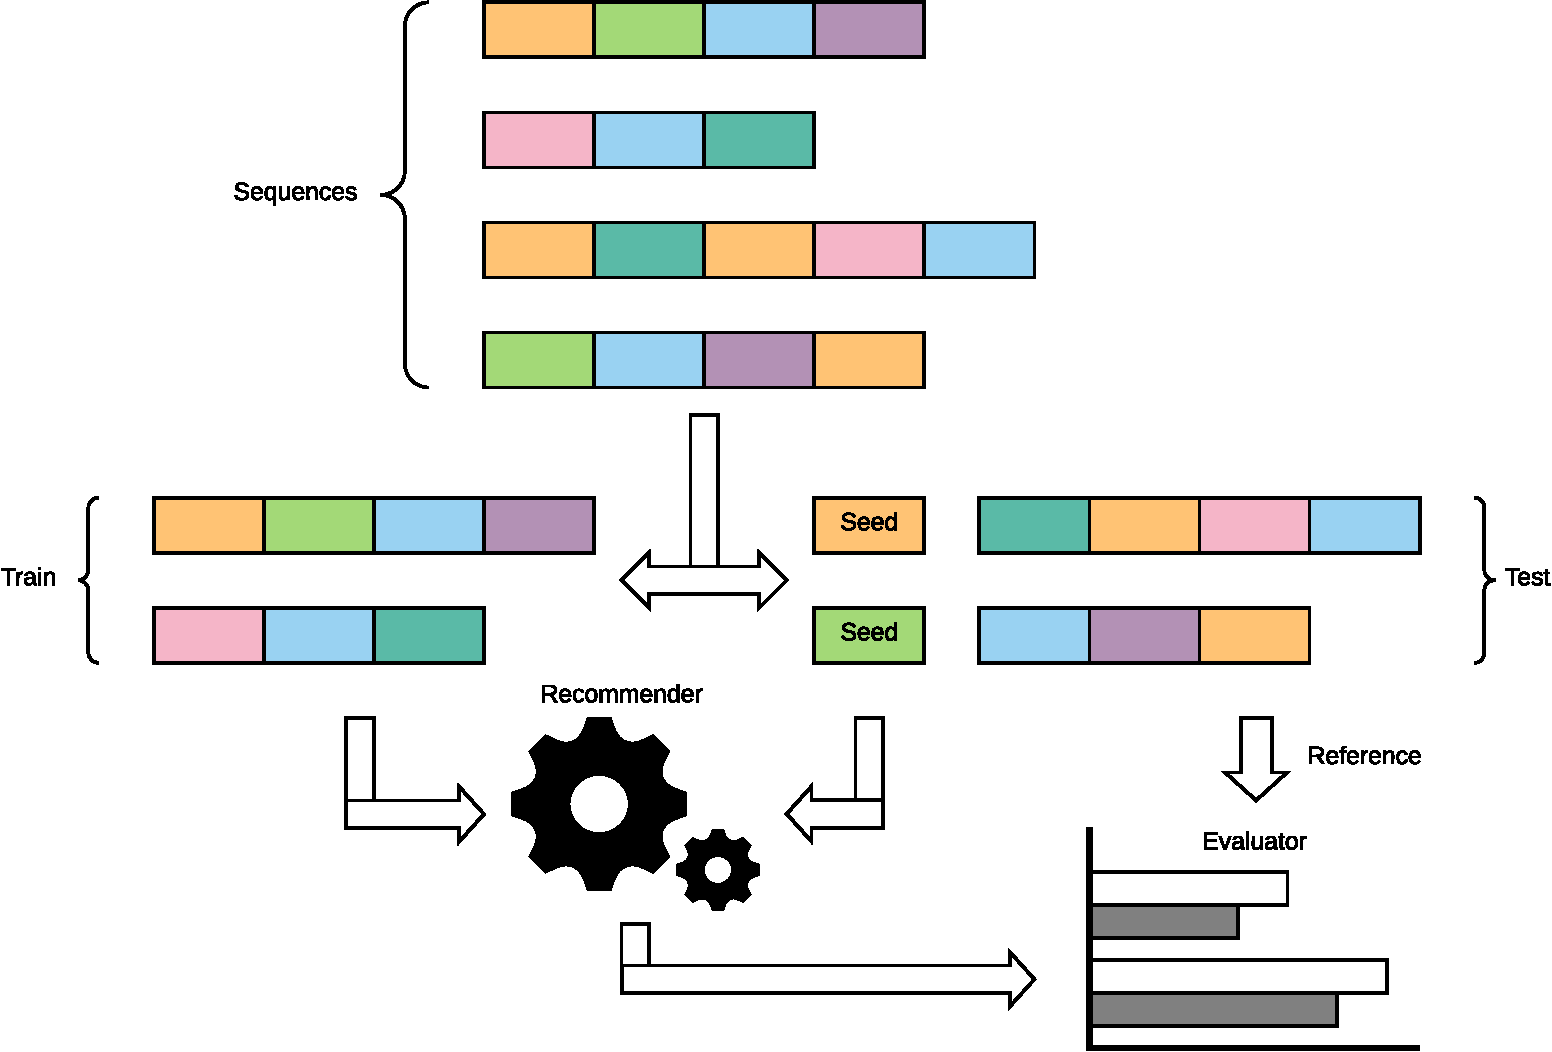
\includegraphics[width=.9\textwidth]{sequeval_protocol.pdf}
\caption[Sequeval evaluation procedure]{An illustration of the evaluation procedure. First, the set of sequences is split between training and test set. Then, the recommender is trained with the sequences available in the training set. Finally, the recommender is asked to generate a sequence for each seed from the test set; such sequences are compared with the corresponding reference sequences.}
\label{seq:fig:sequeval-protocol}
\end{figure}

\subsection{Evaluation Metrics}
\label{seq:sec:metrics}

% General description of the metrics
The second component of Sequeval is a set of eight metrics that we present in the following. In~order to address \ref{seq:itm:rq2}, we include in such set not only classic metrics such as coverage and precision but also less widespread ones such as novelty, diversity, and serendipity. Furthermore, we introduce the metric of perplexity, as it is explicitly designed for characterizing sequences~\cite{Bengio2003}. In contrast, we decided to avoid measuring recall because it is clear that the number of recommended items is often likely to be much lower than the total number of relevant items.

\subsubsection{Coverage}

In general, the coverage of a recommender is a measure that captures the number of items in the catalog over which the system can make suggestions~\cite{Gunawardana2015}. For example, in an online store scenario, it~could represent the percentage of products that are recommended to users in a certain period of time. An algorithm with a higher coverage is generally considered more useful because it better helps users to explore the catalog.

We generate a set of recommended sequences considering as seed the first rating of all sequences in the test set $\mathcal{S}_{test}$ for a recommender that suggests sequences of length $k$. Afterward, we compute the distinct number of items available in the sequences created and we divide the result by the cardinality of the set $\mathcal{I}$.

\begin{equation}
\mathrm{coverage}(k) = \frac{|\bigcup_{\mathbf{s} \in \mathcal{S}_{test}} \mathcal{I}_{\mathrm{sequence}(\mathbf{r}_1, k)}|}{|\mathcal{I}|}
\end{equation}

This metric expresses the percentage of items that the sequence-based recommender can suggest when generating sequences similar to the ones available in the test set and it is strictly related to its cardinality. This approach is similar to the metric of prediction coverage described by Herlocker et al.~\cite{Herlocker2004}.

\subsubsection{Precision}
\label{seq:sec:precision}

Precision is a widespread metric in the context of information retrieval evaluation~\cite{Rijsbergen1979} and it represents the fraction of retrieved documents that are relevant. For a traditional recommender system, precision measures the fraction of recommended items that are relevant for a certain user~\cite{Sarwar2000}. If we consider a sequence-based recommender, it is necessary to compute this metric for each sequence $\mathbf{s} \in \mathcal{S}_{test}$, instead of each user.

\begin{equation}
\mathrm{precision}(k) = \frac{1}{|\mathcal{S}_{test}|} \cdot \sum_{\mathbf{s} \in \mathcal{S}_{test}} \frac{\mathrm{hit}(\mathbf{s'}, \mathbf{\overline{s}})}{\mathrm{min}(|\mathcal{R}_{\mathbf{s'}}|, k)}
\end{equation}

The function $hit : \mathcal{S} \times \mathcal{S} \to \mathbb{N}$ returns the number of items in $\mathbf{\overline{s}}$ that are also available in $\mathbf{s'}$. If the same item is present in $\mathbf{\overline{s}}$ multiple times, it is considered a hit only if it is repeated also in $\mathbf{s'}$. This is an extension to the traditional definition of precision that also considers the fact that an item may appear multiple times inside a sequence.

The number of relevant items is divided by the minimum number between the length of the reference sequence $|\mathcal{R}_{\mathbf{s'}}|$ and the length of the recommended sequence $k$. We decided to adopt this solution to avoid penalizing an algorithm that is evaluated considering reference sequences shorter than the recommended sequences.

\subsubsection{nDPM}

The Normalized Distance-based Performance Metric (nDPM) was originally proposed by Yao in the context of information retrieval~\cite{Yao1995}. The intuition of the author is that in order to compare a system ranking with a reference user ranking, it is necessary to consider all the possible pairs of items available in the system ranking: they can be agreeing, contradictory, or compatible with respect to the user ranking. We decided to adopt such a metric instead of the Normalized Discounted Cumulative Gain (nDCG)~\cite{Jaervelin2002} because, in a sequence of recommendations, it is not necessarily true that the first items are more important than the last ones.

\begin{equation}
\mathrm{nDPM}(k) = \frac{1}{|\mathcal{S}_{test}|} \cdot \sum_{\mathbf{s} \in \mathcal{S}_{test}} \frac{2\,\mathrm{pairs}^-(\mathbf{s'}, \mathbf{\overline{s}}) + \mathrm{pairs}^u(\mathbf{s'}, \mathbf{\overline{s}})}{2\,\mathrm{pairs}(\mathbf{\overline{s}})}
\end{equation}

The function $pairs^- : \mathcal{S} \times \mathcal{S} \to \mathbb{N}$ returns the number of pairs in the sequence $\mathbf{\overline{s}}$ that are in the opposite order with respect to the reference sequence $\mathbf{s'}$. The function $pairs^u : \mathcal{S} \times \mathcal{S} \to \mathbb{N}$ returns the number of pairs in the sequence $\mathbf{\overline{s}}$ for which the ordering is irrelevant, i.e., when at least one of the items is not available in $\mathbf{s'}$ or when at least one of the items is available multiple times in $\mathbf{s'}$. Finally, the function $pairs : \mathcal{S} \to \mathbb{N}$ returns the number of all possible pairs available in the recommended sequence $\mathbf{\overline{s}}$. The pairs are created without considering the ordering of the items inside a pair: for example, if we have the sequence $\langle a, b, c \rangle$, the possible pairs are $(a, b),\allowbreak (a, c),\allowbreak (b, c)$.

The value of this metric will result close to $1$ when the sequences generated by the recommender are contradictory, to $0$ when they have the same ranking, and to $0.5$ when the ordering is irrelevant because they contain different items. A low precision will imply a nDPM very close to $0.5$.

\subsubsection{Diversity}

The metric of sequence diversity included in this framework is inspired by the metric of Intra-List Similarity proposed by Ziegler et al.~\cite{Ziegler2005}. The recommended sequences are considered to be lists of items and the obtained value is not related to their internal ordering. The purpose of this metric is understanding if the sequences contain items that are sufficiently diverse. A higher diversity may be beneficial for the users, as they are encouraged to better explore the catalog~\cite{Noia2014}.

\begin{equation}
\mathrm{diversity}(k) = \frac{1}{|\mathcal{S}_{test}|} \cdot \sum_{\mathbf{s} \in \mathcal{S}_{test}} \frac{\sum_{\forall{i}, \forall{j} : 0 < i < j}^k 1 - \mathrm{sim}(\overline{\iota}_i, \overline{\iota}_j)}{k \times (k - 1)}
\end{equation}

The function $sim : \mathcal{I} \times \mathcal{I} \to [-1, 1]$ is a generic similarity measure between two items. This measure may be taxonomy-driven or content-based: for example, a possible content-based similarity measure is the cosine similarity. The resulting value is a number in the interval $[0, 2]$: higher values represent a higher diversity.

\subsubsection{Novelty}

Vargas et al.~\cite{Vargas2011} suggested that it would be useful to be able to characterize the novelty of the recommendations. They proposed a metric that rewards algorithms capable of identifying items that have a low probability of being already known by a specific user because they belong to the long-tail of the catalog. We have included such metric in our framework to assess whether the items available in the suggested sequences are not too obvious.

\begin{equation}
\mathrm{novelty}(k) = - \frac{1}{|\mathcal{S}_{test}| \times k} \cdot \sum_{\mathbf{s} \in \mathcal{S}_{test}} \sum_{i = 1}^{k} \log_2 \mathrm{freq}(\overline{\iota}_i)
\end{equation}

The function $freq : \mathcal{I} \to [0, 1]$ returns the normalized frequency of a certain item $\iota \in \mathcal{I}$, i.e., the probability of observing that item in a given sequence $\mathbf{s} \in \mathcal{S}_{training}$. We can define the probability of observing the item $\iota$ as the number of ratings related to $\iota$ in the training sequences divided by the total number of ratings available. We also assume that $\log_2(0) \doteq 0$ by definition, to avoid considering as novel items for which we do not have any information, i.e., the items that do not appear in the training sequences.

\subsubsection{Serendipity}

Serendipity can be defined as the capability of identifying items that are both attractive and unexpected~\cite{Gemmis2015b}. Ge et al. proposed to measure the serendipity of a recommender by relying on the precision of the generated lists after having discarded the items that are too obvious~\cite{Ge2010}.

To create a list of obvious items, it is possible to exploit a \emph{primitive} recommender that is a recommender only capable of making obvious suggestions. For example, a primitive recommender could be implemented using the Most Popular (MP) baseline, which is defined in Section~\ref{seq:sec:implementation}. It is reasonable to assume that popular items do not contribute to the serendipity of the recommendations because they are already well known by many users.

By modifying the metric of precision described in Section~\ref{seq:sec:precision}, it is possible to introduce the concept of serendipity in the evaluation of a sequence-based recommender. In this case, the primitive recommender will always create a sequence of length $k$ that contains the items that are have been observed with the highest frequency in the training set.

\begin{equation}
\mathrm{serendipity}(k) = \frac{1}{|\mathcal{S}_{test}|} \cdot \sum_{\mathbf{s} \in \mathcal{S}_{test}} \frac{\mathrm{hit}(\mathbf{s'}, \mathbf{\overline{s}} - \mathbf{\hat{s}})}{\mathrm{min}(|\mathcal{R}_{\mathbf{s'}}|, k)}
\end{equation}

We define $\mathbf{\hat{s}}$ as the sequence generated by the primitive recommender from the same seed of $\mathbf{\overline{s}}$, i.e., $\mathbf{\hat{s}} = \mathrm{primitive}(\mathbf{r}_1, k)$. Moreover, the sequence $\mathbf{\overline{s}} - \mathbf{\hat{s}}$ contains all the ratings related to the items available in $\mathbf{\overline{s}}$ that are not present in $\mathbf{\hat{s}}$. The resulting value will be a number in the interval $[0, 1]$, lower than or equal to precision. The difference between precision and serendipity represents the percentage of obvious items that are correctly suggested.

\subsubsection{Confidence}

The metric of confidence reflects how much the system trusts its own suggestions and it is useful for understanding how robust the learned model is~\cite{Herlocker2000}. It is usually computed as the average probability that the suggested items are correct. This metric expresses the point of view of the recommender, as the probability is reported by the model. Therefore, the metric is always equal to~$1$ with the MP recommender, as it is certain of the predictions.

A sequence-based recommender generates the next item of the sequence by considering all the previous items. For this reason, we can interpret the conditional probability of obtaining a certain item, given the sequence of previous ones, as the confidence that the system has in that suggestion.

\begin{equation}
\mathrm{confidence}(k) = \frac{1}{|\mathcal{S}_{test}| \times k} \cdot \sum_{\mathbf{s} \in \mathcal{S}_{test}} \sum_{i = 1}^k P(\overline{\iota}_i | \overline{\iota}_{i - 1}, \overline{\iota}_{i - 2}, \dotsc)
\end{equation}

We also define $\overline{\iota}_0 \doteq \iota_1$, i.e., the \textit{zero}-th item of the recommended sequence is its seed item. Therefore, this metric is computed by also considering the probability of obtaining the first item $\overline{\iota}_1$, given the seed item of $\mathbf{\overline{s}}$.

\subsubsection{Perplexity}
\label{seq:sec:perplexity}

Perplexity is a widespread metric in the context of neural language modeling evaluation~\cite{Bengio2003}, typically used to measure the quality of the generated phrases. Because there is a strong similarity between creating a sequence of natural language words and sequence of recommended items given an initial seed, perplexity can be also successfully exploited in this context.

This metric can be defined as the exponential in base $2$ of the average negative log-likelihood of the model, i.e., the cross-entropy of the model. For models based on the cross-entropy loss function such as neural networks, the perplexity can also be seen as a measure of convergence of the learning algorithm. Differently from the metric of confidence, the conditional probability $P(\iota_{i + 1} | \iota_i, \iota_{i - 1}, \dotsc)$ is computed considering the items of the test sequence $\mathbf{s}$, and not of the recommended sequence $\mathbf{\overline{s}}$. For this reason, it does not express the point of view of the recommender.

\begin{equation}
\mathrm{perplexity} = 2^{-\frac{1}{\sum_{\mathbf{s} \in \mathcal{S}_{test}} |\mathcal{R}_\mathbf{s}| - 1} \cdot \sum_{\mathbf{s} \in \mathcal{S}_{test}} \sum_{i = 0}^{|\mathcal{R}_\mathbf{s}| - 1} \log_2 P(\iota_{i + 1} | \iota_i, \iota_{i - 1}, \dotsc)}
\end{equation}

Intuitively, the obtained value represents the number of items from which an equivalent random recommender should choose to obtain a similar sequence. The lower is the perplexity, the better is the system under evaluation. Therefore, the perplexity of a random recommender is equal to $|\mathcal{I}|$. If the performance of the recommender is worse than a random one, the perplexity will be higher than $|\mathcal{I}|$: for example, if only one conditional probability is equal to zero, then $\mathrm{perplexity} = +\infty$.

\subsection{Implementation}
\label{seq:sec:implementation}

The third component of Sequeval is \texttt{sequeval}~\cite{Sequeval2018}, a Python implementation of the evaluation framework that is publicly available on GitHub.\footnote{\url{https://github.com/D2KLab/sequeval}} This implementation is based on the protocol presented in Section~\ref{seq:sec:protocol} and it includes the metrics described in Section~\ref{seq:sec:metrics}.

In details, \texttt{sequeval} is a Python package designed following a modular structure, which is graphically represented in Figure~\ref{seq:fig:uml}. For each component, we defined an abstract class and then we realized one or more possible implementations to enable software extensibility.

\begin{figure}
\centering
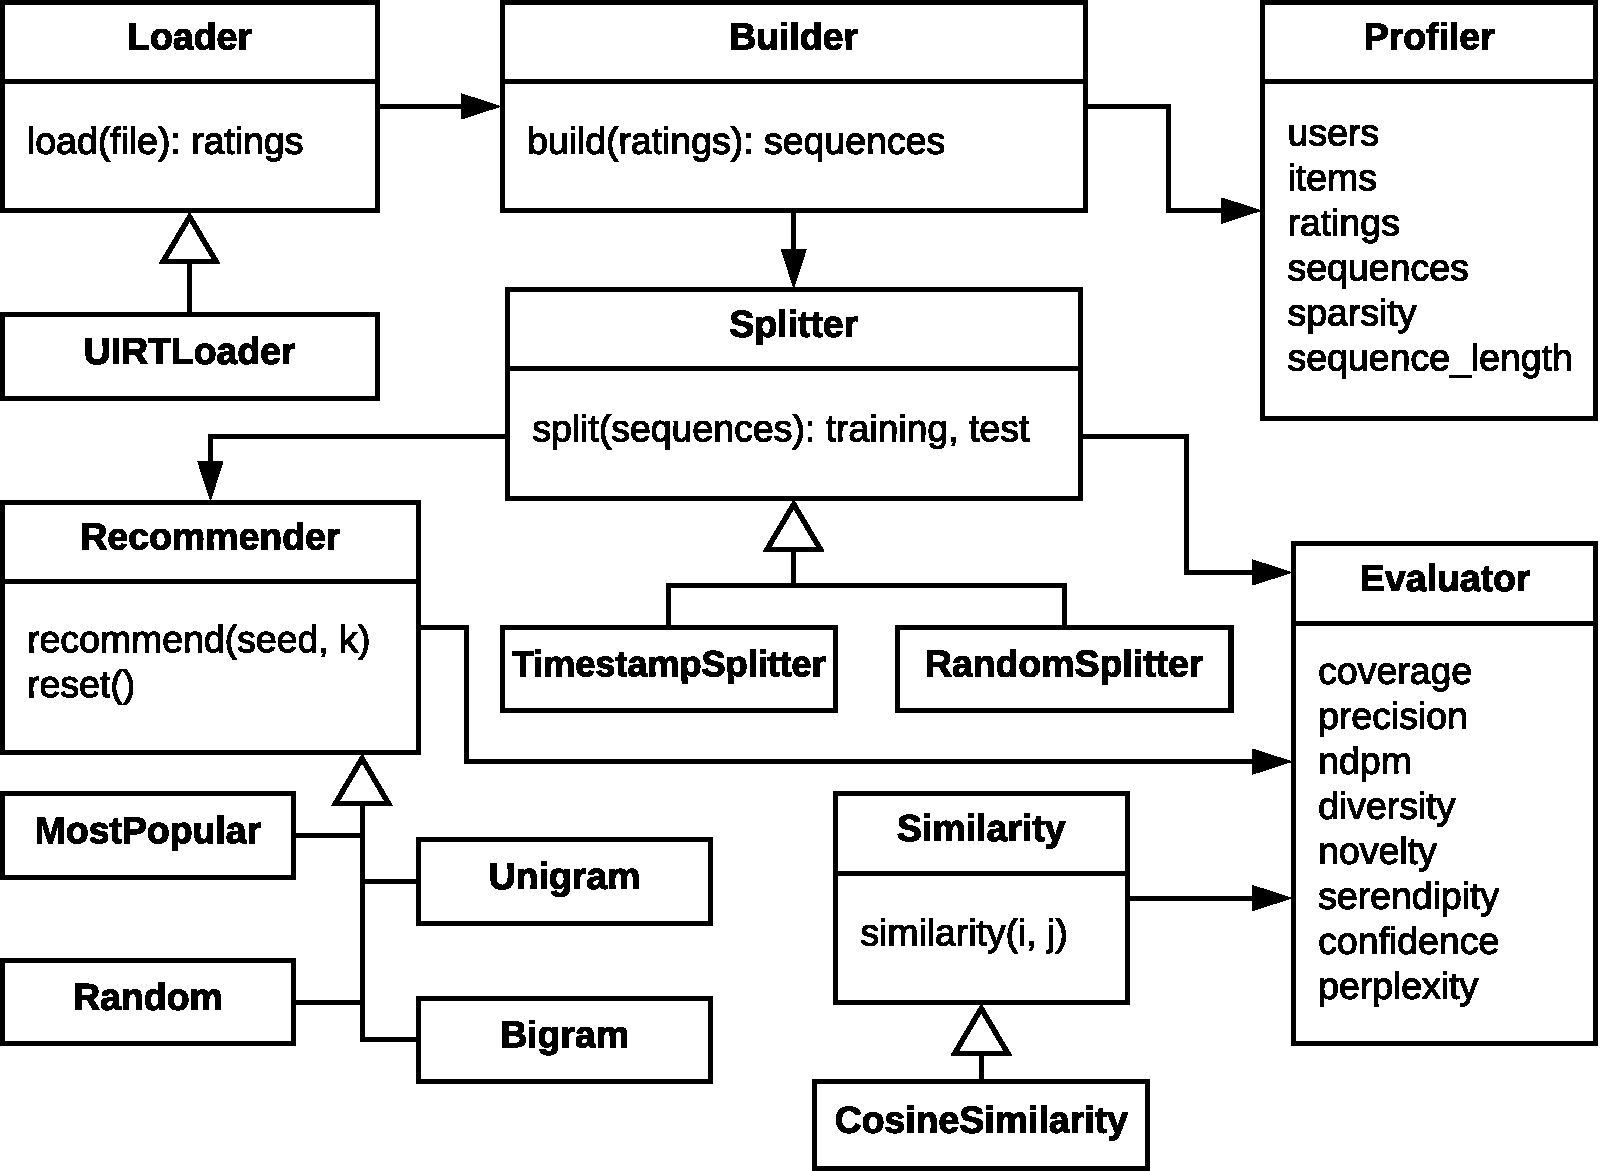
\includegraphics[width=.9\linewidth]{uml}
\caption[UML class diagram of sequeval]{A simplified UML class diagram of \texttt{sequeval}.}
\label{seq:fig:uml}
\end{figure}

The \textit{loader} module is in charge of reading an input file containing user ratings. We have implemented a concrete \textit{loader} capable of processing a textual file in a MovieLens-like format (UIRT), but the support to other formats can be easily added. It is optionally possible to ignore users or items that do not have a minimum number of ratings, in order to avoid data sparsity issues. The \textit{builder} module creates the sequences of items from the initial ratings: ratings from the same user that are distant in time less then a threshold are grouped inside the same sequence. Ratings that do not belong to any sequence are discarded.

The \textit{profiler} module computes some statistics about the generated sequences, for example their average length. The \textit{splitter} module assigns the sequences created by the \textit{builder} to the training and the test sets, according to a random or to a more realistic timestamp-based strategy. It is up to the experimenter deciding the percentage of sequences in the test set.

The \textit{recommender} module includes an abstract class that needs to be implemented by any recommender that relies on this framework, based on the sequence generation logic formalized in Algorithm~\ref{seq:alg:recommend}. The purpose of the abstract class in the \textit{similarity} module is to compute a content-based similarity metric between two items; we have chosen to implement it as a generic cosine-based similarity. Finally, the \textit{evaluator} module computes the measures detailed in Section~\ref{seq:sec:metrics}.

To exploit the proposed framework, it is necessary to realize an implementation of the abstract recommender that must be capable, given the user and the current item of the sequence, of predicting the probabilities for the possible items of being the next one inside the recommended sequence. If the weighted random sampling generation logic is not appropriate, it is possible to override the relative method and to define an alternative recommendation approach.

For obtaining the experimental results, it is necessary to write an evaluation script that relies on this library. We provide a simple evaluation script which can be used to perform different experiments. This script can be easily modified to accommodate novel recommendation techniques.

We also created an extensive test suite achieving the 98\% of code coverage for validating the robustness of our implementation and for better supporting future improvements and developments.% The total development cost of this Python library could be estimated around 40 h.

For demonstrative purposes, we have implemented four baseline recommenders, which are illustrated in the following and represent our answer to \ref{seq:itm:rq3}. These baselines can be interpreted as an adaptation of classic non-personalized recommendation techniques to our sequence-based scenario.

% Baselines
\begin{description}
\item[Most Popular] The MP recommender analyzes the sequences available in the training set to compute the popularity of each item, i.e., the number of times an item appears in the training sequences. Then, at recommendation time, it ignores the seed rating, and it always creates a sequence that contains the MP item as the first rating, the second MP item as the second rating, and so on. More formally, the probability that the item $\iota_i$ will appear in the \textit{i}-th rating of the sequence is $P(\iota_i) = 1$, where $i$ also represents the position of the item in the ranking of the MP ones.
\item[Random] The random recommender simply creates sequences composed of ratings that contain an item randomly sampled from a uniform probability distribution. The seed rating is discarded and the probability of observing the item $\iota_i$ is $P(\iota_i) = 1 / |\mathcal{I}|$, where $|\mathcal{I}|$ represents the number of items available.
\item[Unigram] The unigram recommender can generate sequences that contain ratings with items sampled with a probability proportional to the number of times they were observed in the training sequences. In particular, the probability of observing the item $\iota_i$ is equal to the number of ratings containing $\iota_i$ divided by the total number of ratings available in the training sequences. As with the previous baselines, the seed rating is ignored during the recommendation.
\item[Bigram] The bigram recommender estimates the 1{-st} order transition probabilities among all possible pair of items available in the training sequences. The add-one smoothing technique is exploited to avoid the attribution of a strict zero probability to the pairs that were not observed during the training phase~\cite{Chen1999}. At recommendation time, the seed rating is exploited for selecting the first item, and then each item will influence the choice of the next one. The probability of sampling item $\iota_i$ after item $\iota_{i - 1}$ is equal to the number of times this transition occurred in the training sequences plus one divided by the total number of transitions available.
\end{description}

\section{Experimental Analysis}
\label{seq:sec:analysis}

In this section, we perform an experimental analysis of Sequeval by relying on its implementation described in Section~\ref{seq:sec:implementation} for comparing the behavior of the four baselines with a recommender system based on Conditional Random Fields (CRF)~\cite{Sutton2011} and another one that exploits Recurrent Neural Networks (RNN)~\cite{Goodfellow2016}. The purpose of this comparison is to assess the validity of the framework by conducting an offline evaluation in a realistic scenario. Furthermore, we aim to investigate the efficiency of the proposed approach by analyzing the amount of time required to compute the numerical scores per each recommender system, considering datasets of different sizes.

\subsection{Experimental Setup}
\label{seq:sec:setup}

% Parameters
The main parameters that need to be specified according to our evaluation framework are the $\delta \tau$ value used to generate the sequences, the splitting protocol, and the length of the recommended sequences $k$. The $\delta \tau$ value and the splitting protocol depend on the dataset and they are reported in Section~\ref{seq:sec:datasets}. For performing this empirical analysis, we have decided to exploit the $80\%$ of the dataset for training the recommenders and the remaining $20\%$ for testing purposes. The length of the recommended sequences depends on the specifications of the target application: for this evaluation, we have chosen to set $k = 5$.

% Similarity metric
To compute the metric of diversity, we have selected the cosine similarity among the training sequences as the proximity measure between two items. In fact, we assume that two items are similar if they appear the same number of times inside the same training sequences. Furthermore, we have assumed that if an item is unknown, its similarity with another one is \textit{zero} by definition.

% CRF and RNN
In the following, we provide the rationale for the usage and the implementation details of the two recommenders based on CRF and RNN.

\begin{description}
\item[CRF] We have implemented a CRF-based recommender system using the \texttt{CRFsuite} software package.\footnote{\url{http://www.chokkan.org/software/crfsuite}} Since we are interested in predicting an item given the previous one, we have considered to be feature vectors the training sequences without their last rating and as corresponding output vectors the same sequences without their first rating. We have used the gradient descent algorithm with the L-BFGS method~\cite{Nocedal1980} as the training technique. We have chosen to generate both the state and the transition features that do not occur in the dataset and we have set the maximum number of iterations allowed for the optimization algorithm to $100$.
\item[RNN] We have also experimented with a sequence recommender, originally designed for the tourism domain, based on RNN~\cite{Palumbo2017} that are specifically meant to deal with sequential data. The hyper-parameters of the network have been optimized through a manual search on the validation set in~\cite{Palumbo2017}, obtaining: $\mathrm{n\_layers} = 3$, $\mathrm{dropout} = 0.2$, $\mathrm{learning\_rate} = 0.0001$, $\mathrm{n\_hidden} = 64$, and $\mathrm{n\_epochs} = 10$.
The main difference of RNNs with respect to standard feed-forward neural networks is the presence of a hidden state variable $h_t$, whose value depends both on the input data presented at time $x_t$ and on the previously hidden state $h_{t-1}$~\cite{Goodfellow2016} using loop connections. 
A typical application of RNNs in neural language modeling is the generation of text by recursively applying a ``next word prediction''~\cite{Sutskever2011}. In the same spirit, we address the problem of next item prediction. The probability of the next {rating} given the previous ones $P(\mathbf{r}_{k} | \langle \mathbf{r}_0, \mathbf{r}_1, \dotsc, \mathbf{r}_{k - 1} \rangle)$ is learned during the training process of the neural network without the need for specifying a particular memory window as in Markov models.
\end{description}

For conducting this experimental campaign, we relied on a machine equipped with two 12-cores Intel Xeon processors (E5-2680 v3 at 2.50~GHz) and 128~GB of RAM. However, note that \texttt{sequeval} is a single-threaded application and its memory requirements are actually much lower, around 2.5~GB with the most demanding dataset at our disposal.

\subsection{Datasets}
\label{seq:sec:datasets}

We have performed the experimental analysis considering two different datasets, namely Yes.com and Foursquare. The former is related to the music domain, while the latter deals with check-ins performed at specific POIs.

Because we are interested in modeling sequences, it is important that the temporal information available is actually meaningful. For example, the popular MovieLens datasets~\cite{Harper2015} cannot be exploited for our purposes because the timestamps are associated with the action of assigning a rating on the platform and not with the action of watching a movie. This hypothesis is supported by the fact that, if~we apply Algorithm~\ref{seq:alg:generate} to the MovieLens~1M dataset with $\delta \tau = 1\ \mathrm{h}$, we obtain unrealistic sequences with an average length of about $56$ movies.

The Yes.com and Foursquare datasets are characterized by a different distribution of their items, i.e., songs and venue categories, as it can be observed from Figure~\ref{seq:fig:datasets-barplot}. In particular, Foursquare contains few items that are extremely popular, while Yes.com presents a plot that is smoother. This conclusion is numerically supported by the values of entropy~\cite{Shannon1948} obtained for the two distributions, which are $4.95$ for Foursquare and $6.75$ for Yes.com. Furthermore, the number of sequences available in Foursquare is about $40$ times higher with respect to Yes.com. Table~\ref{seq:tab:datasets-stats} summarizes the number of users, items, ratings, and sequences available in these datasets, which are described in detail in the following sections.

\begin{figure}
\centering
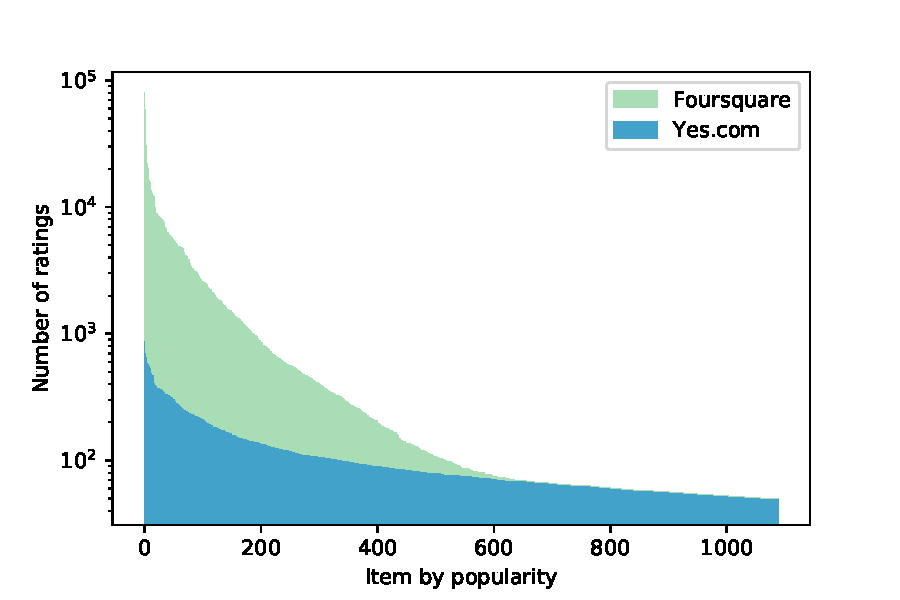
\includegraphics[width=.9\textwidth]{datasets_barplot.pdf}
\caption[Number of ratings per item]{A stacked bar plot with a logarithmic scale representing the number of ratings for each item. Note the different shapes of their long-tail distributions: it is possible to observe that Foursquare has more popular items than Yes.com.}
\label{seq:fig:datasets-barplot}
\end{figure}

\begin{table}
\centering
\begin{tabular}{@{}ccccc@{}}
\toprule
Dataset    & $|\mathcal{U}|$ & $|\mathcal{I}|$ & $|\mathcal{R}|$ & $|\mathcal{S}|$ \\ \midrule
Yes.com    & 1               & 1089            & 118,022         & 10,551          \\
Foursquare & 44,319          & 651             & 1,047,429       & 400,261         \\ \bottomrule
\end{tabular}
\caption[Statistics about the sequences]{The number of users, items, ratings, and sequences after the preprocessing steps. The Yes.com dataset has only one user.}
\label{seq:tab:datasets-stats}
\end{table}

\subsubsection{Yes.com}

This dataset contains several playlists originally collected by Shuo Chen from {Yes.com} in the context of his research on Metric Embedding~\cite{Chen2012}. Such website provided a set of APIs\footnote{\url{http://web.archive.org/web/20150316134941/http://api.yes.com}} for programmatically retrieving songs aired by different radio stations in the United States. By crawling them in the period from December 2010 to May 2011, he managed to obtain $2,840,553$ transitions. Even if {Yes.com} is no longer active, the playlist dataset is publicly available.\footnote{\url{https://www.cs.cornell.edu/~shuochen/lme/data_page.html}}

Yes.com does not include the timestamps, but only the playlists. Therefore, we have assumed that each playlist represents a sequence, as defined in our evaluation framework. In this case, it is not necessary to apply Algorithm~\ref{seq:alg:generate} because the sequences are already available in the dataset in an explicit form. Because a timestamp-based splitting is not feasible, we have selected, for this dataset, a random splitting protocol for dividing the sequences between training and test set.

Since we do not have any information regarding the radio stations, it is necessary to consider the playlists as if they were created by the same user. This approximation is acceptable in the context of sequence recommendation and it is allowed by the evaluation framework. In fact, differently from traditional evaluation approaches, all the metrics that we propose are averaged over the sequences and not over the users. 

Because of the computational complexity of the task, we have randomly reduced the complete dataset $10$ times its original size and we have pruned the songs that appear less than $50$ times.

\subsubsection{Foursquare}

The second dataset that we have selected for performing the experimental evaluation of the framework is similar to the one described in~\cite{Palumbo2017} and it was created following the same protocol.

We collected the check-ins performed by the users of the Foursquare Swarm mobile application\footnote{\url{https://www.swarmapp.com}} and publicly shared on Twitter from the Twitter API. Then, we retrieved the category of the place associated with the check-in thanks to the Foursquare API. For this reason, the items of the dataset are represented by the venue categories available in the Foursquare taxonomy.\footnote{\url{https://developer.foursquare.com/docs/resources/categories}} The collection phase lasted from October to December 2017.

To avoid exploiting the interactions generated by automated scripts, we have discarded the users that performed multiple check-ins in less than one minute. We have also pruned the check-ins associated with the venue categories that are usually not of interest for a tourist, for example the ones related to workplaces. For generating the sequences more efficiently, we decided to also remove the users that have performed less than $10$ check-ins in total.

We have set the $\delta \tau$ parameter of the evaluation framework to $8$ h. Regarding the splitting protocol, we have selected the timestamp-based one, considering the timestamp associated with the first rating as the timestamp of the sequence.

\subsection{Results}

Table~\ref{seq:tab:results-yes} summarizes the figures of the evaluation conducted with Yes.com. The MP recommender achieved a fair precision, but at the price of a very low coverage, because its predictions are deterministic.
Unsurprisingly, the lowest precision and the highest novelty and diversity are associated with the random recommender. In contrast, the unigram, the bigram, and the CRF recommenders obtained comparable scores of precision, but the bigram is the most appealing of these three techniques, because of its lower perplexity and higher novelty.

\begin{table}
\centering
\begin{tabular}{@{}ccccccc@{}}
\toprule
Metric      & MP        & Random & Unigram & Bigram & CRF    & RNN    \\ \midrule
Coverage    & 0.0046    & 1.0000 & 0.9945  & 1.0000 & 0.9991 & 0.9458 \\
Precision   & 0.0503    & 0.0090 & 0.0127  & 0.0103 & 0.0190 & 0.0782 \\
nDPM        & 0.5007    & 0.5000 & 0.5000  & 0.5000 & 0.5000 & 0.4986 \\
Diversity   & 0.6925    & 0.9900 & 0.9815  & 0.9854 & 0.9788 & 0.9052 \\
Novelty     & 7.2383    & 10.380 & 9.7349  & 10.315 & 9.8449 & 9.5762 \\
Serendipity & 0.0000    & 0.0089 & 0.0107  & 0.0095 & 0.0179 & 0.0706 \\
Confidence  & 1.0000    & 0.0009 & 0.0016  & 0.0011 & 0.0020 & 0.0123 \\
Perplexity  & $+\infty$ & 1089.0 & 848.96  & 637.53 & 747.33 & 183.49 \\ \bottomrule
\end{tabular}
\caption[Experimental results with Yes.com]{The results of the baselines and both CRF and RNN with Yes.com.}
\label{seq:tab:results-yes}
\end{table}

We can observe that the RNN recommender achieved the highest precision and the lowest perplexity, resulting to be the most promising algorithm for future online experimentations. Its nDPM is slightly lower than $0.5$, meaning that the items are usually predicted in the correct order. We can also observe that its serendipity is close to the value of precision: for this reason, it is possible to assume that most of the sequences are not obvious.

Table~\ref{seq:tab:results-foursquare} lists, instead, the results obtained with Foursquare. In this case, the MP recommender system accounted for the highest precision, meaning that the top-$5$ items are extremely widespread, but, as usual, its coverage is very limited, and it achieved the lowest novelty. On the other hand, the random recommender scored the lowest precision, and the highest coverage and novelty. The differences among the unigram, the bigram, and the CRF recommenders are more striking than in the previous experiment: with this dataset, the unigram accounted for higher precision because of the popularity of some items, while the bigram for the lowest perplexity.

\begin{table}
\centering
\begin{tabular}{@{}ccccccc@{}}
\toprule
Metric      & MP        & Random & Unigram & Bigram & CRF    & RNN    \\ \midrule
Coverage    & 0.0077    & 1.0000 & 0.9616  & 1.0000 & 0.9677 & 0.5069 \\
Precision   & 0.2259    & 0.0080 & 0.0774  & 0.0607 & 0.0754 & 0.0962 \\
nDPM        & 0.4998    & 0.5000 & 0.4994  & 0.4998 & 0.4993 & 0.4991 \\
Diversity   & 0.9194    & 0.9971 & 0.9616  & 0.9777 & 0.9621 & 0.9469 \\
Novelty     & 4.6056    & 12.300 & 7.1421  & 9.0216 & 7.3710 & 6.8374 \\
Serendipity & 0.0000    & 0.0060 & 0.0256  & 0.0230 & 0.0252 & 0.0365 \\
Confidence  & 1.0000    & 0.0015 & 0.0171  & 0.0140 & 0.0179 & 0.0264 \\
Perplexity  & $+\infty$ & 651.00 & 141.41  & 122.99 & 147.49 & 140.39 \\ \bottomrule
\end{tabular}
\caption[Experimental results with Foursquare]{The results of the baselines and both CRF and RNN with Foursquare.}
\label{seq:tab:results-foursquare}
\end{table}

The RNN recommender system obtained the second-best precision and perplexity, resulting in a good compromise if we are interested in optimizing both these metrics. Its fair coverage and the low value of serendipity are other hints of the fact that the Foursquare dataset contains few items that are very popular: this characteristic was, in fact, learned and exploited by the recommender.

Finally, we report in Table~\ref{seq:tab:results-efficiency} the amount of time needed for computing the previously described evaluation metrics per recommendation algorithm with the Foursquare and Yes.com datasets. We observe that in the worst case, the evaluation framework was able to conduct an experimental campaign in a few hours. The metric of diversity was the most computationally expensive one because of the time needed to compute the cosine similarity. This fact is particularly evident if we consider the seconds spent to evaluate the random recommender with the Foursquare dataset.

\begin{table}
\centering
\begin{tabular}{@{}cccccccc@{}}
\toprule
Dataset & Div. & MP & Random & Unigram & Bigram & CRF & RNN \\ \midrule
Yes.com & Yes & 0.84 & 4.25 & 3.97 & 4.05 & 963.65 & 66.04 \\
Yes.com & No & 0.78 & 1.14 & 0.98 & 1.05 & 865.17 & 60.68 \\
Foursquare & Yes & 15.88 & 1326.31 & 58.64 & 101.73 & 4096.78 & 1223.26 \\
Foursquare & No & 13.75 & 24.63 & 13.05 & 16.78 & 3989.17 & 1194.52 \\ \bottomrule
\end{tabular}
\caption[Time to evaluate the algorithms]{The time in seconds required to evaluate different algorithms with our framework. We do not consider the time for training the CRF and RNN models. To improve the efficiency of the framework it is possible to avoid computing the computationally expensive metric of diversity.}
\label{seq:tab:results-efficiency}
\end{table}

As expected, the baseline recommenders are less demanding with respect to the CRF and RNN models. However, this analysis is beyond the scope of this work, as we are only interested in optimizing the evaluation framework. If we do not consider the metric of diversity, we observe that the time required for the evaluation phase is linear with respect to the size of the dataset.

\subsection{Discussion}

In the following, we will analyze the results of the empirical analysis to justify the answers to the research questions that were provided in Section~\ref{seq:sec:sequence-based} and in Section~\ref{seq:sec:sequeval}. In particular, our main aim is to explain why it is necessary to rely on a multicriteria framework that includes several metrics to evaluate a sequence-based recommender system.

% Why we need items, users, and timestamps
In Section~\ref{seq:sec:sequence-based} we have introduced the concept of rating and we have defined it considering three different elements: an item, a user, and a timestamp. The idea of associating a user with an item is the basic principle of almost every recommender, while the timestamp is necessary in order to introduce a temporal dimension, and, therefore, the possibility of creating and suggesting sequences, as proposed in \ref{seq:itm:rq1}. Nevertheless, we have successfully applied our evaluation framework in an experiment based on the Yes.com dataset, which does not include any user. Even though a {more} general use case has been considered during its formalization, it is possible to also exploit it in other scenarios, still obtaining an interesting picture of the recommenders under evaluation.

% Why so many metrics
As described in Section~\ref{seq:sec:metrics}, our answer to \ref{seq:itm:rq2} is an evaluation framework that includes eight different metrics, capable of capturing the various characteristics of the algorithms available. For~example, even if the precision of the MP recommender system is very high when tested with Foursquare, we can immediately discard it because of its low coverage. In the same way, the interesting values of diversity and novelty achieved by the random recommender are associated with an unacceptable score of perplexity.

In Table~\ref{seq:tab:metrics-interpretation} we present an interpretation of the metrics available in the framework. These descriptions are meant to offer a human understanding of the results of the offline evaluation. It is worth noticing that these metrics consider only some of the properties of a recommender system~\cite{Gunawardana2015}. However, it is our opinion that those properties are the most salient ones that can be analyzed in our context, without realizing a live system.

\begin{table}
\centering
\begin{tabular}{@{}ll@{}}
\toprule
Metric      & Interpretation                                                  \\ \midrule
Coverage    & The percentage of items that are recommended in the evaluation  \\
Precision   & The percentage of items that are correctly recommended          \\
nDPM        & The correctness of the ordering inside the sequences            \\
Diversity   & How diverse are the items inside the sequences                  \\
Novelty     & How unexpected are the recommended items                        \\
Serendipity & The percentage of non-obvious items that are correct            \\
Confidence  & The confidence that the recommender has about its predictions   \\
Perplexity  & How much the recommender is ``surprised'' by the test sequences \\ \bottomrule
\end{tabular}
\caption[Interpretation of the metrics]{A human readable interpretation of the metrics.}
\label{seq:tab:metrics-interpretation}
\end{table}

The different characteristics of the datasets exploited during the empirical analysis are reflected in their respective figures. In particular, while the values of precision obtained by the random recommender in the two experiments are comparable, the figures associated with both MP and unigram methods are dramatically different. This fact suggests that Foursquare contains a few items that are extremely popular, as it was already clear from Figure~\ref{seq:fig:datasets-barplot}.

On the other hand, the RNN recommender obtained, with both datasets, comparable values of precision, but a very different coverage. For this reason, we can suppose that this approach, differently from the CRF recommender, is capable of better adapting itself to the characteristics of the dataset. The~fact that we can draw such {a }conclusion supports the validity of Sequeval.

Furthermore, we have observed that the amount of time required to compute the evaluation metrics is linear with respect to the dataset size, if we do not consider the metric of diversity. In fact, the computational cost of the cosine similarity was too elevated when we analyzed the behavior of the random recommender with a more demanding dataset. However, because of the modular structure of \texttt{sequeval}, it is easy to avoid computing the metric of diversity for such a recommender.

% What are the properties of each baseline
In line with \ref{seq:itm:rq3}, we have described in Section~\ref{seq:sec:implementation} four different baseline recommenders. From the results of the experiments, it is possible to observe that the values obtained by some of them are fixed. For example, the MP recommender will always achieve a serendipity equal to $0$, and a confidence equal to $1$. Its perplexity is usually $+\infty$, if at least one of the recommended sequences is incorrect. The items suggested are, in fact, considered obvious by definition, and the algorithm is certain of the recommendation because its behavior is deterministic. In a similar way, the perplexity of the random recommender is equal to the total number of items available, i.e., $|\mathcal{I}|$, because of the definition of perplexity provided in Section~\ref{seq:sec:perplexity}.

These two baselines are methods commonly exploited in the literature for evaluating recommender systems. Additionally, we have proposed two techniques better suited for the sequence recommendation problem. The unigram recommender is similar to the MP one, but it is non-deterministic, and it obtained a higher novelty. In contrast, the bigram recommender is the most complex baseline, because it considers the previous item to suggest the next one. For this reason, it always achieved the lowest perplexity among the baselines considered.

\section{Conclusion}
\label{seq:sec:conclusion}

% Summary
In this chapter, we have discussed the problem of recommending sequences of items tailored to the needs of a certain user. We have introduced an offline evaluation framework, called Sequeval, capable of handling this novel family of recommender systems in an offline scenario and we have developed an implementation of it that is publicly available on GitHub. We have included in such a framework an evaluation protocol and eight different metrics, to better capture the characteristics of the algorithms considered.

% Empirical analysis
We have performed an empirical analysis of Sequeval by relying on it for conducting a comparison among four baselines, a CRF recommender, and an RNN-based one. The results have highlighted the fact that this framework is flexible, as it can be successfully applied in non-standard recommendation scenarios, such as with Yes.com, and complete, because of the different metrics included that consider several dimensions of the recommended sequences. In addition, we have observed that the RNN recommender system can effectively adapt itself to the characteristics of the training dataset. This conclusion supports the validity of Sequeval as a tool for conducting an offline experimentation.

The formal definitions provided in Section~\ref{seq:sec:sequence-based} have been conceived as an extension of the seminal works on recommenders capable of recommending sequences. For this reason, it is possible to set the length of the recommended sequences to $1$ if we are interested in obtaining a single item. In a similar way, the item included in the seed rating can be exploited in order to set the context of the recommendation, but it can also be ignored if we want a sequence only based on the target user.
